\documentclass[aspectratio=43]{beamer}
% Theme works only with a 4:3 aspect ratio
\usetheme{CSCS}

\usepackage{tikz}
\usetikzlibrary{calc,shapes.multipart,chains,arrows,automata}

% define footer text
\newcommand{\footlinetext}{P. Crosetto}

% Select the image for the title page
\newcommand{\picturetitle}{cscs_images/image3.pdf}
%\newcommand{\picturetitle}{cscs_images/image5.pdf}
%\newcommand{\picturetitle}{cscs_images/image6.pdf}


% Please use the predifined colors:
% cscsred, cscsgrey, cscsgreen, cscsblue, cscsbrown, cscspurple, cscsyellow, cscsblack, cscswhite

\author{Paolo Crosetto, C2SM/CSCS}
\title{STL overview}
\subtitle{Advanced C++ for HPC}
\date{\today}

\begin{document}

% TITLE SLIDE
\cscstitle

% EMPTY SLIDE
%% \begin{frame}
%% \end{frame}

% TABLE OF CONTENT SLIDE
% All options for table of contents:
% currentsection, currentsubsection, firstsection=xx, hideallsubsections, hideothersubsections, part=xx, pausesections, pausesubsections, sections=xx, sections={xx-yy}, sections={xx,yy}
%\cscstableofcontents[hideallsubsections]{Title}
\cscstableofcontents{Standard Template Library (STL) Overview}

\begin{frame}[fragile]{Material}
  Clone the github repo
\begin{verbatim}
git clone https://github.com/crosetto/examples_cpp.git
\end{verbatim}
  Most of the code snippets shown are avaliable in
\begin{verbatim}
examples_cpp/Code/STL/
\end{verbatim}
  Exercices are in
\begin{verbatim}
examples_cpp/Exercices/STL/
\end{verbatim}
\end{frame}

\begin{frame}[fragile]\frametitle{STL}
  STL components:
  \begin{itemize}
  \item containers
  \item iterators
  \item algorithms
  \item tuple
  \item utility
  \item threads
  \item smart pointers
  \item regexp
  \item I/O
  \item exceptions
  \item More ...
  \end{itemize}
\end{frame}

\begin{frame}[fragile]\frametitle{STL}
  We will focus in this section on:
  \begin{itemize}
  \item containers,
  \item iterators,
  \item algorithms,
  \item tuple.
  \end{itemize}
\end{frame}

\section{Containers}

\begin{frame}[fragile]\frametitle{std::array}
  std::array is as an \emph{aggregate}.
  \begin{itemize}
  \item no overheads w.r.t. C arrays
  \item static size (runtime error when out-of-bounds if using \verb1at()1)
  \item constant-time access, linear-time swap
  \item can be constexpr
  \item swap does a deep copy
  \end{itemize}
  \begin{Cpplisting}[: array.cpp]{}
constexpr array<int, 5> arr_{0,1,2,3,4};
static_assert(arr_[2] == get<2>(arr_) == 2, "error");
static_assert(arr_.size() == 5, "error");
static_assert(arr_.back() == 4, "error");
static_assert(arr_.front() == 0, "error");
array<int, 2> arr1_{1,0}, arr2_{0,1};
arr2_.swap(arr1_); //deep copy!!
  \end{Cpplisting}
\end{frame}

\begin{frame}[fragile]\frametitle{std::vector}
  \begin{itemize}
  \item resizable set of elements of the same type
  \item faster pushing/popping at the end (constant)
  \item contiguous in memory (fast access/iteration, may be expensive to resize)
  \item constant time random access
  \item different implementation for \verb1std::vector<bool>1
  \item \verb1capacity1, \verb1shrink_to_fit1, \verb1reserve1
  \end{itemize}
  \begin{Cpplisting}[: vector\_capacity.cpp]{}
std::vector< char > v_(2001);
std::cout<<v_.capacity()<<" "; // 2001
v_.push_back('b');
std::cout<<v_.capacity()<<" "; // 4002
v_.shrink_to_fit(); // non-binding
std::cout<<v_.capacity()<<"\n"; // 2002
v_.reserve(2004); v_.push_back('d');
std::cout<<v_.capacity()<<"\n"; // 2004
  \end{Cpplisting}
\end{frame}

\begin{frame}[fragile]\frametitle{std::vector of bool, std::bitset}
  \begin{itemize}
  \item special optimized implementation (stores coalescing bits)
  \item cannot take address of elements
  \item not thread safe (as opposed as all other containers)
  \item use \verb1std::bitset1 if the size is static
  \item \verb1std::bitset1 is constexpr constructable
  \end{itemize}
\begin{onlyenv}<1>
  \begin{Cpplisting}[: vector\_bool.cpp]{}
std::vector< bool > v_={true, false, true};
std::cout<<v_.size()<<"\n";
constexpr std::bitset<3> b_(0b101);
std::cout<<sizeof(v_)<<" != "<<sizeof(b_)<<"\n";
std::cout<<b_[2]<<" = "<<v_[2]<<"\n";
static_assert(b_[1]==0, "");
  \end{Cpplisting}
\end{onlyenv}
\begin{onlyenv}<2>
  \begin{Cpplisting}[: vector\_bool.cpp]{}
std::vector< bool > v_={true, false, true};
std::cout<<v_.size()<<"\n"; // 3
constexpr std::bitset<3> b_(0b101);
std::cout<<sizeof(v_)<<" != "<<sizeof(b_)<<"\n"; // 3 =! 8
std::cout<<b_[2]<<" = "<<v_[2]<<"\n"; // 1 = 1
static_assert(b_[1]==0, "");
  \end{Cpplisting}
\end{onlyenv}
\end{frame}

\begin{frame}[fragile]\frametitle{std::deque}
  \verb1std::dequeue1: double ended queue, push and pop from both sides
  \begin{itemize}
  \item similar to \verb1std::vector1 but:
  \item not contiguous in memory
  \item efficiently resizable on both ends
  \item constant time random access
  \end{itemize}
\end{frame}

\begin{frame}[fragile]\frametitle{deque vs vector}
\begin{onlyenv}<1>
  \begin{Cpplisting}[: deque.cpp]{}
std::deque< int > l_(1e8);
for(auto i=1; i < 1e8; i++){
  l_.push_back(8);
}
  \end{Cpplisting}
  \begin{Cpplisting}[: vector\_vs\_deque.cpp]{}
std::vector< int > l_(1e8);
for(auto i=1; i < 1e8; i++){
  l_.push_back(8);
}
  \end{Cpplisting}
\end{onlyenv}

\begin{onlyenv}<2->
  \begin{Cpplisting}[: deque.cpp]{}
std::deque< int > l_(1e5);
for(auto i=1; i < 1e5; i++){
  l_.insert(l_.begin(), 8);
}
  \end{Cpplisting}
  \begin{Cpplisting}[: vector\_vs\_deque.cpp]{}
std::vector< int > l_(1e5);
for(auto i=1; i < 1e5; i++){
  l_.insert(l_.begin(), 8);
}
  \end{Cpplisting}
\end{onlyenv}
\uncover<3>{
  \begin{itemize}
  \item use deque when inserting at the beginning
  \end{itemize}
  }
\end{frame}

\begin{frame}[fragile]\frametitle{std::forward\_list}
  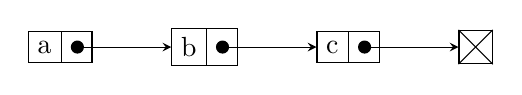
\begin{tikzpicture}[list/.style={rectangle split, rectangle split parts=2,
        draw, rectangle split horizontal}, >=stealth, start chain]

    \node[list,on chain] (A) {a};
    \node[list,on chain] (B) {b};
    \node[list,on chain] (C) {c};
    \node[on chain,draw,inner sep=6pt] (D) {};
    \draw (D.north east) -- (D.south west);
    \draw (D.north west) -- (D.south east);
    \draw[*->] let \p1 = (A.two), \p2 = (A.center) in (\x1,\y2) -- (B);
    \draw[*->] let \p1 = (B.two), \p2 = (B.center) in (\x1,\y2) -- (C);
    \draw[*->] let \p1 = (C.two), \p2 = (C.center) in (\x1,\y2) -- (D);
  \end{tikzpicture}

  \begin{itemize}
  \item linked list of elements of the same type
  \item efficient resizing or removal anywhere in the list (constant)
  \item non contiguous in memory
  \item slow random access (linear)
  \item \verb1std::list1 same thing, but doubly linked list.
  \end{itemize}
\end{frame}

\begin{frame}[fragile]\frametitle{list vs vector}
  \begin{Cpplisting}[: vector\_vs\_list.cpp]{}
std::vector< int > l_(1e5);

for(auto i=0; i < 1e5; i++){
  l_.insert(l_.begin()+2*i, 8);
}
  \end{Cpplisting}

  \begin{Cpplisting}[: list.cpp]{}
std::list< int > l_(1e5);

for(auto i=l_.begin(); i != l_.end(); i++){
  l_.insert(i, 8);
}
  \end{Cpplisting}
  \uncover<2>{
    Use list:
    \begin{itemize}
    \item when inserting/removing in the middle of the container
    \item when the containers are large
    \item when the elements size is big
    \end{itemize}
    \alert{Most of the times STL vectors are much faster!}
  }

\end{frame}

\begin{frame}[fragile]\frametitle{std::queue, std::stack, std::priority\_queue}
  \begin{itemize}
    \item they are container adaptors (use other containers underneeth)
    \item \verb1std::queue1: FIFO, push into one end and pop from the other
    \item \verb1std::stack1: FILO, push and pop into/from one end
    \item \verb1std::priority_queue1
      \begin{itemize}
      \item ordered container, get the largest value in constant time
      \item slow insertion/removal (logarithmic)
      \end{itemize}
  \end{itemize}
\end{frame}

\begin{frame}[fragile]\frametitle{Associative containers}
  \begin{itemize}
    \item \verb1std::map1
      \begin{itemize}
        \item collection of key-value pairs, with a unique key
      \end{itemize}
    \item \verb1std::set1
      \begin{itemize}
        \item holds unique objects
        \item like \verb1std::map1 in which the key is also the element
      \end{itemize}
    \item \verb1std::multiset1 \verb1std::multimap1
      allow multiple keys with equivalent value
    \item The default version of associative containers is \emph{ordered} (using a \verb1Compare1 template parameter). Search/insertion/removal in logarithmic time.
    \item \emph{Unordered} versions (since C++11): search/insertion/removal in average constant time.
  \end{itemize}
\end{frame}


\begin{frame}[fragile]\frametitle{map and set}
  \begin{Cpplisting}[: map.cpp]{}
std::map< std::string, double > m_;
m_.insert(std::make_pair("first", 0.));
m_.insert(std::make_pair("second", 1.));
m_.insert(std::make_pair("third", 1.));
m_.insert(std::make_pair("third", 10.));
double val=m_.find("third")->second;
std::cout<<val<<"\n"; // 1.
std::cout<<"size: "<<m_.size()<<"\n"; // 3
  \end{Cpplisting}

  \begin{Cpplisting}[: set.cpp]{}
std::set< double > m_;
m_.insert( 0. );
m_.insert( 1. );
m_.insert( 1. );
auto val=m_.find(1.);
std::cout<<*val<<"\n"; // 1.
std::cout<<"size: "<<m_.size()<<"\n"; // 2
  \end{Cpplisting}
  \uncover<2>{
    \begin{columns}
      \begin{column}{0.6\textwidth}
        \centering{Associative containers:}
    \begin{itemize}
    \item Usually implemented as binary trees
    \end{itemize}
      \end{column}
      \begin{column}{0.7\textwidth}
        \begin{itemize}
        \item Not in performance-critical regions
        \item Optimized for searching by key
        \end{itemize}
      \end{column}
    \end{columns}
  }

\end{frame}


\begin{frame}[fragile]\frametitle{Emplace}

  \begin{Cpplisting}[: emplace signature]{}
template< class... Args >
iterator emplace( const_iterator pos, Args&&... args );
  \end{Cpplisting}
Inserts a new element into the container directly before pos
  \begin{Cpplisting}[: emplace.cpp]{}
struct my_class{
  my_class(my_class const&){std::cout<<"Copy\n";};
  my_class(int, double){std::cout<<"Construct\n";};
};
    \end{Cpplisting}
\begin{itemize}
  \item \verb1emplace_back1
  \item \verb1emplace1
\end{itemize}
\begin{onlyenv}<1>
\begin{Cpplisting}[: emplace.cpp]{}
int main(){
  std::vector<my_class> m;
  m.reserve(2);
  m.push_back( my_class(1,2.) );
  m.push_back( my_class(1,2.) );
}
\end{Cpplisting}
\end{onlyenv}
\begin{onlyenv}<2>
\begin{Cpplisting}[: emplace.cpp]{}
int main(){
  std::vector<my_class> m;
  m.reserve(2);
  m.push_back( my_class(1,2.) ); // construct and copy
  m.push_back( my_class(1,2.) ); // construct and copy
}
\end{Cpplisting}
\end{onlyenv}
\begin{onlyenv}<3>
\begin{Cpplisting}[: emplace.cpp]{}
int main(){
  std::vector<my_class> m;
  m.reserve(2);
  m.emplace_back( 1,2. );
  m.emplace_back( 1,2. );
}
\end{Cpplisting}
\end{onlyenv}
\begin{onlyenv}<4>
\begin{Cpplisting}[: emplace.cpp]{}
int main(){
  std::vector<my_class> m;
  m.reserve(2);
  m.emplace_back( 1,2. ); // construct
  m.emplace_back( 1,2. ); // construct
}
\end{Cpplisting}
\end{onlyenv}
\begin{onlyenv}<5>
\begin{Cpplisting}[: emplace.cpp]{}
int main(){
  std::vector<my_class> m;
  m.reserve(2);
  m.emplace_back( 1,2. ); // construct
  m.emplace( m.begin(),1,2. ); // ??
}
    \end{Cpplisting}
\end{onlyenv}
\end{frame}

\section{Allocator}

\begin{frame}[fragile]\frametitle{allocator}
  Almost all STL containers have an allocator template parameter.
  Can be used to
  \begin{itemize}
    \item customize the storage allocation policy (cf. example with std::vector)
    \item customize the container for specific types of memory
  \end{itemize}
  since C++11:
  \begin{itemize}
  \item simplified the API for custom allocators
  \item guaranteed that each container holds the instance of its allocator (\alert{stateful allocator possible})
  \end{itemize}
\end{frame}


\begin{frame}[fragile]\frametitle{allocator}
  Example of stateless user-defined allocator
  \begin{Cpplisting}[: heap.cpp]{}
template<typename T>
struct my_allocator{
  using value_type=T;
  T* allocate (int n, allocator<void>::const_pointer hint=0){
    if(n<100)
      return static_cast<T*>(malloc(n*sizeof(T)));
    else throw(bad_alloc());
  }
  void deallocate (T* p, int n){free(p);}
};

main(){
  vector<int,  my_allocator<int> > q_({0,1,2});
  assert(q_[2]==2);
  //vector<int,  my_allocator<int> > q_(101); //throws bad_alloc
}
  \end{Cpplisting}
\end{frame}

\begin{frame}[fragile]\frametitle{Exercice}
  Modify the allocator on the previous slide
  (you can find it in \verb~cpp_examples/Exercices/STL/allocator~), so that it allocates on the
  stack instead of the heap.

\end{frame}


\begin{frame}[fragile]\frametitle{Solution}
  We can allocate on the stack
  \begin{Cpplisting}[: stack.cpp]{}
template<typename T>
struct my_allocator{
  using value_type=T;
  T* allocate (int n, allocator<void>::const_pointer hint=0){
    if(n<100)
      return data; else throw(bad_alloc());
  }
  void deallocate (T* p, int n){/*RAII*/}
  T data[100];
};

main(){
  vector<int,  my_allocator<int> > q_({0,1,2});
  assert(q_[2]==2);
  //vector<int,  my_allocator<int> > q_(101); //throws bad_alloc
}
  \end{Cpplisting}
\end{frame}

\section{Iterators}

\begin{frame}[fragile]\frametitle{Iterators}
  We reviewed all STL containers. They work with \emph{iterators}

  \alert{Why?}
  Not all all STL containers are accessible by index (e.g. \verb1std::list1)

  Iterators provide a generic way to traverse all the types of container

  \begin{Cpplisting}[: iterators definition]{}
struct Container<T>::iterator{
  iterator(const& iterator) //copy
  void operator =(const& iterator) //assign
  iterator operator ++(); // pre-increment
  iterator operator ++(int); // post-increment
  bool operator ==(iterator); // comparison
  bool operator !=(iterator); // comparison
  T operator *(); // dereference
  T * operator -> (); // dereference
};
  \end{Cpplisting}
\end{frame}

\begin{frame}[fragile]\frametitle{Types of Iterators}
  \begin{itemize}
  \item input (read, increment)
  \item output (write, increment)
  \item forward (also multistep increment)
  \item bidirectional (also decrements)
  \item random (also random access)
  \end{itemize}
  \alert{STL algorithms work with iterators}
  \begin{onlyenv}<1>
  \begin{Cpplisting}[: iterators simple example]{}
vector< int > v1_({1,6,2,7,3,5,4});
vector< int > v2_(v1_.begin(), v1_.end());


.
  \end{Cpplisting}
  \end{onlyenv}
  \begin{onlyenv}<2>
  \begin{Cpplisting}[: iterators simple example]{}
vector< int > v1_({1,6,2,7,3,5,4});
vector< int > v2_(max_element(v1_.begin(), v1_.end()), v1_.end());

.
  \end{Cpplisting}
  \end{onlyenv}
  \begin{onlyenv}<3->
  \begin{Cpplisting}[: iterators simple example]{}
vector< int > v1_({1,6,2,7,3,5,4});
vector< int > v2_(max_element(v1_.begin(), v1_.end()), v1_.end());
for(auto i : v2_)
cout<<i<<" ";
  \end{Cpplisting}
  \end{onlyenv}
  \uncover<4>{outputs 7 3 5 4}
\end{frame}


\begin{frame}[fragile]\frametitle{Generic API}
  \begin{center}
    Forward iterator:\\
\only<1>{
    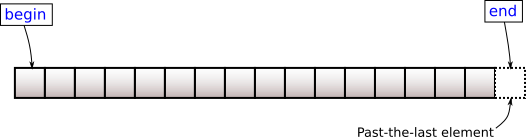
\includegraphics[width=0.7\textwidth]{cpp_course/Images/range-begin-end.png}\\
}
\only<2>{
    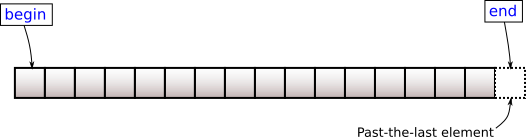
\includegraphics[width=0.3\textwidth]{cpp_course/Images/range-begin-end.png}\\
}
    \begin{onlyenv}<2>
    \begin{Cpplisting}[: reverse\_iterator.cpp]{}
std::vector<int> v{0,1,2,3};
for(auto i=v.begin(); i!=v.end(); ++i)
  std::cout<<*i<<" "; // 0 1 2 3
  \end{Cpplisting}
\end{onlyenv}
    Reverse iterator:\\
    \only<1>{
    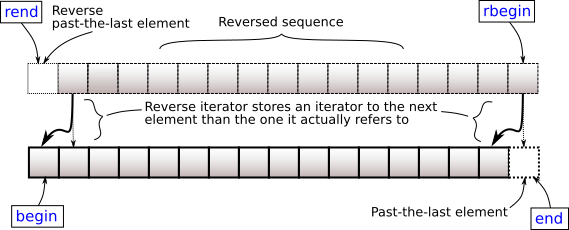
\includegraphics[width=0.7\textwidth]{cpp_course/Images/range-rbegin-rend.png}
    }
    \only<2>{
    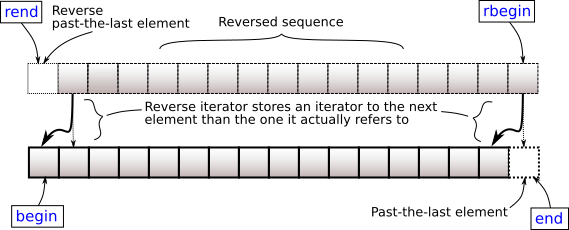
\includegraphics[width=0.3\textwidth]{cpp_course/Images/range-rbegin-rend.png}
    }
    \begin{onlyenv}<2>
    \begin{Cpplisting}[: reverse\_iterator.cpp]{}
std::vector<int> v{0,1,2,3};
for(auto i=v.rbegin(); i!=v.rend(); ++i)
  std::cout<<*i<<" "; // 3 2 1 0
  \end{Cpplisting}
\end{onlyenv}
  \end{center}
\end{frame}


\begin{frame}[fragile]\frametitle{Move Iterator}
  \begin{onlyenv}<1>
  \begin{Cpplisting}[: move\_iterator.cpp]{}
struct my_class{
  my_class() = default;
  my_class(my_class const&){std::cout<<"Copy\n";};
  my_class(my_class &&){std::cout<<"Move\n";};
};

int main(){
  std::vector<my_class> v(1);
  auto it = v.begin();
  auto moved=my_class(*it);
}
  \end{Cpplisting}
Calls the copy constructor
  \end{onlyenv}

  \begin{onlyenv}<2>
  \begin{Cpplisting}[: move\_iterator.cpp]{}
struct my_class{
  my_class() = default;
  my_class(my_class const&){std::cout<<"Copy\n";};
  my_class(my_class &&){std::cout<<"Move\n";};
};

int main(){
  std::vector<my_class> v(1);
  auto it = make_move_iterator(v.begin());
  auto moved=my_class(*it);
}
  \end{Cpplisting}
Calls the move constructor
    \end{onlyenv}
\end{frame}

\begin{frame}[fragile]\frametitle{Iterators invalidation}
  The iterators for an \verb1std::vector1 get invalidated when inserting/erasing elements
  \emph{before} the iteration point, or when the vector is resized:

  \begin{onlyenv}<1>
  \begin{Cpplisting}[: vector\_invalidation.cpp]{}
int t=1;
std::list< int > l_(10);
for(auto i=l_.begin(); i != l_.end(); i++){
  l_.insert(i, t); // OK
}
  \end{Cpplisting}
  \end{onlyenv}
  \begin{onlyenv}<2-3>
  \begin{Cpplisting}[: vector\_invalidation.cpp]{}
int t=1;
std::vector< int > l_(10);
for(auto i=l_.begin(); i != l_.end(); i++){
  l_.insert(i, t); // segfaults
}
  \end{Cpplisting}
  \end{onlyenv}

  \begin{onlyenv}<4>
  \begin{Cpplisting}[: vector\_invalidation.cpp]{}
int t=1;
std::vector< int > l_(10);
for(auto i=l_.begin(); i != l_.end(); i+=2){
  i=l_.insert(i, t);
}
  \end{Cpplisting}
  \end{onlyenv}

  \uncover<3->{because the \alert{end() iterator gets moved at every iteration}.

    and because the \alert{iterator i gets invalidated}.}

  \uncover<4->{we can safely use the iterator \alert{returned by insert}.}

\end{frame}


\begin{frame}[fragile]\frametitle{Iterators invalidation}
  STL List:

  \vspace{1cm}
  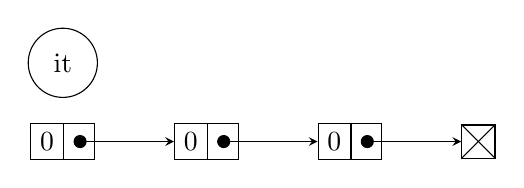
\begin{tikzpicture}[list/.style={rectangle split, rectangle split parts=2,
        draw, rectangle split horizontal}, >=stealth, start chain]

    \node[list,on chain] (A) {0};
    \node[state] (It) [above of=A] {it};
    \node[list,on chain] (B) {0};
    \node[list,on chain] (C) {0};
    \node[on chain,draw,inner sep=6pt] (D) {};
    \draw (D.north east) -- (D.south west);
    \draw (D.north west) -- (D.south east);
    \draw[*->] let \p1 = (A.two), \p2 = (A.center) in (\x1,\y2) -- (B);
    \draw[*->] let \p1 = (B.two), \p2 = (B.center) in (\x1,\y2) -- (C);
    \draw[*->] let \p1 = (C.two), \p2 = (C.center) in (\x1,\y2) -- (D);
  \end{tikzpicture}

  \vspace{1cm}

  Iterators do not get invalidated

\end{frame}

\begin{frame}[fragile]\frametitle{Iterators invalidation}
  STL List:

  \vspace{1cm}

  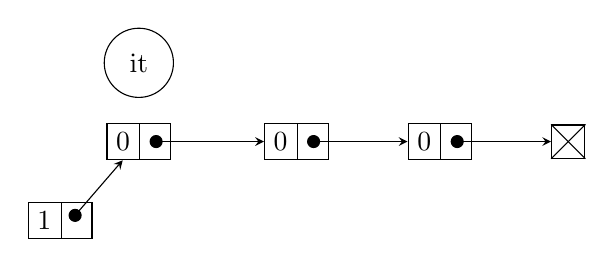
\begin{tikzpicture}[list/.style={rectangle split, rectangle split parts=2,
        draw, rectangle split horizontal}, >=stealth, start chain]

    \node[list,on chain] (S) {1};
    \node[list,on chain] (A) [above of=S] {0};
    \node[state] (It) [above of=A] {it};
    \node[list,on chain] (B) [right of=A] {0};
    \node[list,on chain] (C) {0};
    \node[on chain,draw,inner sep=6pt] (D) {};
    \draw (D.north east) -- (D.south west);
    \draw (D.north west) -- (D.south east);
    \draw[*->] let \p1 = (S.two), \p2 = (S.center) in (\x1,\y2) -- (A);
    \draw[*->] let \p1 = (A.two), \p2 = (A.center) in (\x1,\y2) -- (B);
    \draw[*->] let \p1 = (B.two), \p2 = (B.center) in (\x1,\y2) -- (C);
    \draw[*->] let \p1 = (C.two), \p2 = (C.center) in (\x1,\y2) -- (D);
  \end{tikzpicture}

  \vspace{1cm}

  Iterators do not get invalidated
\end{frame}

\begin{frame}[fragile]\frametitle{Iterators invalidation}
  STL List:

    \vspace{1cm}

  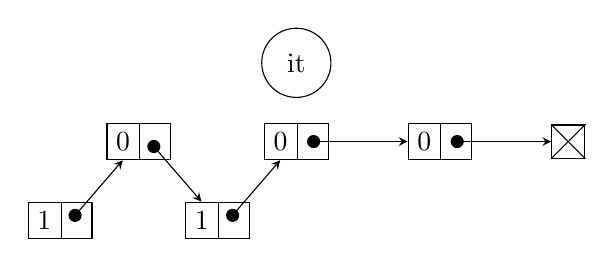
\begin{tikzpicture}[list/.style={rectangle split, rectangle split parts=2,
        draw, rectangle split horizontal}, >=stealth, start chain]

    \node[list,on chain] (S) {1};
    \node[list,on chain] (A) [above of=S]  {0};
    \node[list,on chain] (E) [below of=A]  {1};
    \node[list,on chain] (B) [right of=A]  {0};
    \node[state] (It) [above of=B] {it};
    \node[list,on chain] (C) {0};
    \node[on chain,draw,inner sep=6pt] (D) {};
    \draw (D.north east) -- (D.south west);
    \draw (D.north west) -- (D.south east);
    \draw[*->] let \p1 = (S.two), \p2 = (S.center) in (\x1,\y2) -- (A);
    \draw[*->] let \p1 = (A.two), \p2 = (A.center) in (\x1,\y2) -- (E);
    \draw[*->] let \p1 = (E.two), \p2 = (E.center) in (\x1,\y2) -- (B);
    \draw[*->] let \p1 = (B.two), \p2 = (B.center) in (\x1,\y2) -- (C);
    \draw[*->] let \p1 = (C.two), \p2 = (C.center) in (\x1,\y2) -- (D);
  \end{tikzpicture}

    \vspace{1cm}

  Iterators do not get invalidated
\end{frame}

\begin{frame}[fragile]\frametitle{Iterators invalidation}
  STL List:

  \vspace{1cm}

  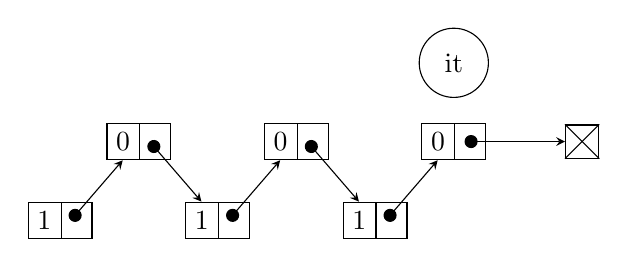
\begin{tikzpicture}[list/.style={rectangle split, rectangle split parts=2,
        draw, rectangle split horizontal}, >=stealth, start chain]

    \node[list,on chain] (S) {1};
    \node[list,on chain] (A) [above of=S]  {0};
    \node[list,on chain] (E) [below of=A]  {1};
    \node[list,on chain] (B) [right of=A]  {0};
    \node[list,on chain] (F) [below of=B]  {1};
    \node[list,on chain] (C) [right of=B] {0};
    \node[state] (It) [above of=C] {it};
    \node[on chain,draw,inner sep=6pt] (D) {};
    \draw (D.north east) -- (D.south west);
    \draw (D.north west) -- (D.south east);
    \draw[*->] let \p1 = (S.two), \p2 = (S.center) in (\x1,\y2) -- (A);
    \draw[*->] let \p1 = (A.two), \p2 = (A.center) in (\x1,\y2) -- (E);
    \draw[*->] let \p1 = (E.two), \p2 = (E.center) in (\x1,\y2) -- (B);
    \draw[*->] let \p1 = (B.two), \p2 = (B.center) in (\x1,\y2) -- (F);
    \draw[*->] let \p1 = (F.two), \p2 = (F.center) in (\x1,\y2) -- (C);
    \draw[*->] let \p1 = (C.two), \p2 = (C.center) in (\x1,\y2) -- (D);
  \end{tikzpicture}

    \vspace{1cm}

  Iterators do not get invalidated
\end{frame}

\begin{frame}\frametitle{Iterators invalidation}
  STL vector:

  \vspace{1cm}

  {
      {\color{red} \tiny 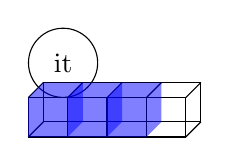
\begin{tikzpicture}[scale=0.5]
    \node[state] (It) at(0.5,1.5) {it};
    \foreach \x in{0,...,4}
             {
               \draw (\x ,0,1) -- (\x ,1,1);
               \draw (\x ,1,1) -- (\x ,1,0);
             }
    \foreach \x in{0,...,3}
             {
               \draw (\x,0,0)--(\x+1,0,0);
             }
             \draw (0,0 ,1) -- (4,0 ,1);
             \draw (0,1 ,1) -- (4,1 ,1);
             \draw (4,0 ,1) -- (4,0 ,0);
             \draw (4,0,0 ) -- (4,1,0 );
             \draw (0,1,0 ) -- (4,1,0 );
             \draw (0,1,0 ) -- (0,0,0 );
             \draw (0,0,0 ) -- (0,0,1 );


             \fill[opacity=0.5,blue]
                (0,0,1) -- (1,0,1)
             -- (1,0,1) -- (1,1,1)
             -- (1,1,1) -- (0,1,1)
             -- (0,1,1) -- (0,0,1) -- cycle;
             \fill[opacity=0.5,blue]
                (0,1,0) -- (1,1,0)
             -- (1,1,0) -- (1,1,1)
             -- (1,1,1) -- (0,1,1)
             -- (0,1,1) -- (0,1,0) -- cycle;
             \fill[opacity=0.5,blue]
                (1,0,0) -- (1,1,0)
             -- (1,1,0) -- (1,1,1)
             -- (1,1,1) -- (1,0,1)
             -- (1,0,1) -- (1,0,0) -- cycle;

             \fill[opacity=0.5,blue]
                (1,0,1) -- (2,0,1)
             -- (2,0,1) -- (2,1,1)
             -- (2,1,1) -- (1,1,1)
             -- (1,1,1) -- (1,0,1) -- cycle;
             \fill[opacity=0.5,blue]
                (1,1,0) -- (2,1,0)
             -- (2,1,0) -- (2,1,1)
             -- (2,1,1) -- (1,1,1)
             -- (1,1,1) -- (1,1,0) -- cycle;
             \fill[opacity=0.5,blue]
                (2,0,0) -- (2,1,0)
             -- (2,1,0) -- (2,1,1)
             -- (2,1,1) -- (2,0,1)
             -- (2,0,1) -- (2,0,0) -- cycle;

             \fill[opacity=0.5,blue]
                (2,0,1) -- (3,0,1)
             -- (3,0,1) -- (3,1,1)
             -- (3,1,1) -- (2,1,1)
             -- (2,1,1) -- (2,0,1) -- cycle;
             \fill[opacity=0.5,blue]
                (2,1,0) -- (3,1,0)
             -- (3,1,0) -- (3,1,1)
             -- (3,1,1) -- (2,1,1)
             -- (2,1,1) -- (2,1,0) -- cycle;
             \fill[opacity=0.5,blue]
                (3,0,0) -- (3,1,0)
             -- (3,1,0) -- (3,1,1)
             -- (3,1,1) -- (3,0,1)
             -- (3,0,1) -- (3,0,0) -- cycle;

  \end{tikzpicture}
}
  }

\end{frame}


\begin{frame}\frametitle{Iterators invalidation}
  STL vector:

  \vspace{1cm}

  {
      {\color{red} \tiny 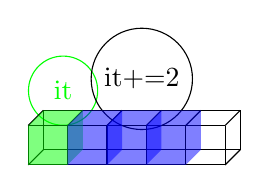
\begin{tikzpicture}[scale=0.5]
          {\color{green}\node[state] (It) at(0.5,1.5) {it};}
          \node[state] (It) at(2.5,1.8) {it+=2};

     \foreach \x in{0,...,5}
             {
               \draw (\x ,0,1) -- (\x ,1,1);
               \draw (\x ,1,1) -- (\x ,1,0);
             }
    \foreach \x in{0,...,4}
             {
               \draw (\x,0,0)--(\x+1,0,0);
             }
             \draw (0,0 ,1) -- (5,0 ,1);
             \draw (0,1 ,1) -- (5,1 ,1);
             \draw (5,0 ,1) -- (5,0 ,0);
             \draw (5,0,0 ) -- (5,1,0 );
             \draw (0,1,0 ) -- (5,1,0 );
             \draw (0,1,0 ) -- (0,0,0 );
             \draw (0,0,0 ) -- (0,0,1 );


             \fill[opacity=0.5,green]
                (0,0,1) -- (1,0,1)
             -- (1,0,1) -- (1,1,1)
             -- (1,1,1) -- (0,1,1)
             -- (0,1,1) -- (0,0,1) -- cycle;
             \fill[opacity=0.5,green]
                (0,1,0) -- (1,1,0)
             -- (1,1,0) -- (1,1,1)
             -- (1,1,1) -- (0,1,1)
             -- (0,1,1) -- (0,1,0) -- cycle;
             \fill[opacity=0.5,green]
                (1,0,0) -- (1,1,0)
             -- (1,1,0) -- (1,1,1)
             -- (1,1,1) -- (1,0,1)
             -- (1,0,1) -- (1,0,0) -- cycle;

             \fill[opacity=0.5,blue]
                (1,0,1) -- (2,0,1)
             -- (2,0,1) -- (2,1,1)
             -- (2,1,1) -- (1,1,1)
             -- (1,1,1) -- (1,0,1) -- cycle;
             \fill[opacity=0.5,blue]
                (1,1,0) -- (2,1,0)
             -- (2,1,0) -- (2,1,1)
             -- (2,1,1) -- (1,1,1)
             -- (1,1,1) -- (1,1,0) -- cycle;
             \fill[opacity=0.5,blue]
                (2,0,0) -- (2,1,0)
             -- (2,1,0) -- (2,1,1)
             -- (2,1,1) -- (2,0,1)
             -- (2,0,1) -- (2,0,0) -- cycle;

             \fill[opacity=0.5,blue]
                (2,0,1) -- (3,0,1)
             -- (3,0,1) -- (3,1,1)
             -- (3,1,1) -- (2,1,1)
             -- (2,1,1) -- (2,0,1) -- cycle;
             \fill[opacity=0.5,blue]
                (2,1,0) -- (3,1,0)
             -- (3,1,0) -- (3,1,1)
             -- (3,1,1) -- (2,1,1)
             -- (2,1,1) -- (2,1,0) -- cycle;
             \fill[opacity=0.5,blue]
                (3,0,0) -- (3,1,0)
             -- (3,1,0) -- (3,1,1)
             -- (3,1,1) -- (3,0,1)
             -- (3,0,1) -- (3,0,0) -- cycle;

             \fill[opacity=0.5,blue]
                (3,0,1) -- (4,0,1)
             -- (4,0,1) -- (4,1,1)
             -- (4,1,1) -- (3,1,1)
             -- (3,1,1) -- (3,0,1) -- cycle;
             \fill[opacity=0.5,blue]
                (3,1,0) -- (4,1,0)
             -- (4,1,0) -- (4,1,1)
             -- (4,1,1) -- (3,1,1)
             -- (3,1,1) -- (3,1,0) -- cycle;
             \fill[opacity=0.5,blue]
                (4,0,0) -- (4,1,0)
             -- (4,1,0) -- (4,1,1)
             -- (4,1,1) -- (4,0,1)
             -- (4,0,1) -- (4,0,0) -- cycle;

        \end{tikzpicture}
}
  }

  \vspace{1cm}

  Iterators get invalidated
\end{frame}


\begin{frame}\frametitle{Iterators invalidation}
  STL vector:

  \vspace{1cm}

  {
      {\color{red} \tiny 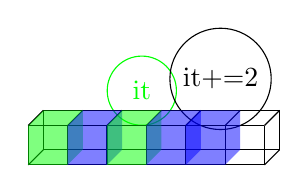
\begin{tikzpicture}[scale=0.5]
          {\color{green}\node[state] (It) at(2.5,1.5) {it};}
          \node[state] (It) at(4.5,1.8) {it+=2};
   \foreach \x in{0,...,6}
             {
               \draw (\x ,0,1) -- (\x ,1,1);
               \draw (\x ,1,1) -- (\x ,1,0);
             }
    \foreach \x in{0,...,5}
             {
               \draw (\x,0,0)--(\x+1,0,0);
             }
             \draw (0,0 ,1) -- (6,0 ,1);
             \draw (0,1 ,1) -- (6,1 ,1);
             \draw (6,0 ,1) -- (6,0 ,0);
             \draw (6,0,0 ) -- (6,1,0 );
             \draw (0,1,0 ) -- (6,1,0 );
             \draw (0,1,0 ) -- (0,0,0 );
             \draw (0,0,0 ) -- (0,0,1 );



             \fill[opacity=0.5,green]
                (0,0,1) -- (1,0,1)
             -- (1,0,1) -- (1,1,1)
             -- (1,1,1) -- (0,1,1)
             -- (0,1,1) -- (0,0,1) -- cycle;
             \fill[opacity=0.5,green]
                (0,1,0) -- (1,1,0)
             -- (1,1,0) -- (1,1,1)
             -- (1,1,1) -- (0,1,1)
             -- (0,1,1) -- (0,1,0) -- cycle;
             \fill[opacity=0.5,green]
                (1,0,0) -- (1,1,0)
             -- (1,1,0) -- (1,1,1)
             -- (1,1,1) -- (1,0,1)
             -- (1,0,1) -- (1,0,0) -- cycle;

             \fill[opacity=0.5,blue]
                (1,0,1) -- (2,0,1)
             -- (2,0,1) -- (2,1,1)
             -- (2,1,1) -- (1,1,1)
             -- (1,1,1) -- (1,0,1) -- cycle;
             \fill[opacity=0.5,blue]
                (1,1,0) -- (2,1,0)
             -- (2,1,0) -- (2,1,1)
             -- (2,1,1) -- (1,1,1)
             -- (1,1,1) -- (1,1,0) -- cycle;
             \fill[opacity=0.5,blue]
                (2,0,0) -- (2,1,0)
             -- (2,1,0) -- (2,1,1)
             -- (2,1,1) -- (2,0,1)
             -- (2,0,1) -- (2,0,0) -- cycle;

             \fill[opacity=0.5,green]
                (2,0,1) -- (3,0,1)
             -- (3,0,1) -- (3,1,1)
             -- (3,1,1) -- (2,1,1)
             -- (2,1,1) -- (2,0,1) -- cycle;
             \fill[opacity=0.5,green]
                (2,1,0) -- (3,1,0)
             -- (3,1,0) -- (3,1,1)
             -- (3,1,1) -- (2,1,1)
             -- (2,1,1) -- (2,1,0) -- cycle;
             \fill[opacity=0.5,green]
                (3,0,0) -- (3,1,0)
             -- (3,1,0) -- (3,1,1)
             -- (3,1,1) -- (3,0,1)
             -- (3,0,1) -- (3,0,0) -- cycle;

             \fill[opacity=0.5,blue]
                (3,0,1) -- (4,0,1)
             -- (4,0,1) -- (4,1,1)
             -- (4,1,1) -- (3,1,1)
             -- (3,1,1) -- (3,0,1) -- cycle;
             \fill[opacity=0.5,blue]
                (3,1,0) -- (4,1,0)
             -- (4,1,0) -- (4,1,1)
             -- (4,1,1) -- (3,1,1)
             -- (3,1,1) -- (3,1,0) -- cycle;
             \fill[opacity=0.5,blue]
                (4,0,0) -- (4,1,0)
             -- (4,1,0) -- (4,1,1)
             -- (4,1,1) -- (4,0,1)
             -- (4,0,1) -- (4,0,0) -- cycle;


             \fill[opacity=0.5,blue]
                (4+0,0,1) -- (4+1,0,1)
             -- (4+1,0,1) -- (4+1,1,1)
             -- (4+1,1,1) -- (4+0,1,1)
             -- (4+0,1,1) -- (4+0,0,1) -- cycle;
             \fill[opacity=0.5,blue]
                (4+0,1,0) -- (4+1,1,0)
             -- (4+1,1,0) -- (4+1,1,1)
             -- (4+1,1,1) -- (4+0,1,1)
             -- (4+0,1,1) -- (4+0,1,0) -- cycle;
             \fill[opacity=0.5,blue]
                (4+1,0,0) -- (4+1,1,0)
             -- (4+1,1,0) -- (4+1,1,1)
             -- (4+1,1,1) -- (4+1,0,1)
             -- (4+1,0,1) -- (4+1,0,0) -- cycle;

        \end{tikzpicture}
}
  }

  \vspace{1cm}

  Iterators get invalidated

\end{frame}


\begin{frame}\frametitle{Iterators invalidation}
  STL vector:

  \vspace{1cm}

  {
    {\color{red} \tiny 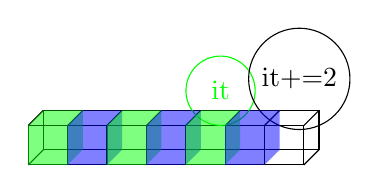
\begin{tikzpicture}[scale=0.5]
    \foreach \x in{0,...,7}
             {
               \draw (\x ,0,1) -- (\x ,1,1);
               \draw (\x ,1,1) -- (\x ,1,0);
             }
    \foreach \x in{0,...,6}
             {
               \draw (\x,0,0)--(\x+1,0,0);
             }
             \draw (0,0 ,1) -- (7,0 ,1);
             \draw (0,1 ,1) -- (7,1 ,1);
             \draw (7,0 ,1) -- (7,0 ,0);
             \draw (7,0,0 ) -- (7,1,0 );
             \draw (0,1,0 ) -- (7,1,0 );
             \draw (0,1,0 ) -- (0,0,0 );
             \draw (0,0,0 ) -- (0,0,1 );

             {\color{green}\node[state] (It) at(4.5,1.5) {it};}
             \node[state] (It) at(6.5,1.8) {it+=2};

             \fill[opacity=0.5,green]
                (0,0,1) -- (1,0,1)
             -- (1,0,1) -- (1,1,1)
             -- (1,1,1) -- (0,1,1)
             -- (0,1,1) -- (0,0,1) -- cycle;
             \fill[opacity=0.5,green]
                (0,1,0) -- (1,1,0)
             -- (1,1,0) -- (1,1,1)
             -- (1,1,1) -- (0,1,1)
             -- (0,1,1) -- (0,1,0) -- cycle;
             \fill[opacity=0.5,green]
                (1,0,0) -- (1,1,0)
             -- (1,1,0) -- (1,1,1)
             -- (1,1,1) -- (1,0,1)
             -- (1,0,1) -- (1,0,0) -- cycle;

             \fill[opacity=0.5,blue]
                (1,0,1) -- (2,0,1)
             -- (2,0,1) -- (2,1,1)
             -- (2,1,1) -- (1,1,1)
             -- (1,1,1) -- (1,0,1) -- cycle;
             \fill[opacity=0.5,blue]
                (1,1,0) -- (2,1,0)
             -- (2,1,0) -- (2,1,1)
             -- (2,1,1) -- (1,1,1)
             -- (1,1,1) -- (1,1,0) -- cycle;
             \fill[opacity=0.5,blue]
                (2,0,0) -- (2,1,0)
             -- (2,1,0) -- (2,1,1)
             -- (2,1,1) -- (2,0,1)
             -- (2,0,1) -- (2,0,0) -- cycle;

             \fill[opacity=0.5,green]
                (2,0,1) -- (3,0,1)
             -- (3,0,1) -- (3,1,1)
             -- (3,1,1) -- (2,1,1)
             -- (2,1,1) -- (2,0,1) -- cycle;
             \fill[opacity=0.5,green]
                (2,1,0) -- (3,1,0)
             -- (3,1,0) -- (3,1,1)
             -- (3,1,1) -- (2,1,1)
             -- (2,1,1) -- (2,1,0) -- cycle;
             \fill[opacity=0.5,green]
                (3,0,0) -- (3,1,0)
             -- (3,1,0) -- (3,1,1)
             -- (3,1,1) -- (3,0,1)
             -- (3,0,1) -- (3,0,0) -- cycle;

             \fill[opacity=0.5,blue]
                (3,0,1) -- (4,0,1)
             -- (4,0,1) -- (4,1,1)
             -- (4,1,1) -- (3,1,1)
             -- (3,1,1) -- (3,0,1) -- cycle;
             \fill[opacity=0.5,blue]
                (3,1,0) -- (4,1,0)
             -- (4,1,0) -- (4,1,1)
             -- (4,1,1) -- (3,1,1)
             -- (3,1,1) -- (3,1,0) -- cycle;
             \fill[opacity=0.5,blue]
                (4,0,0) -- (4,1,0)
             -- (4,1,0) -- (4,1,1)
             -- (4,1,1) -- (4,0,1)
             -- (4,0,1) -- (4,0,0) -- cycle;


             \fill[opacity=0.5,green]
                (4+0,0,1) -- (4+1,0,1)
             -- (4+1,0,1) -- (4+1,1,1)
             -- (4+1,1,1) -- (4+0,1,1)
             -- (4+0,1,1) -- (4+0,0,1) -- cycle;
             \fill[opacity=0.5,green]
                (4+0,1,0) -- (4+1,1,0)
             -- (4+1,1,0) -- (4+1,1,1)
             -- (4+1,1,1) -- (4+0,1,1)
             -- (4+0,1,1) -- (4+0,1,0) -- cycle;
             \fill[opacity=0.5,green]
                (4+1,0,0) -- (4+1,1,0)
             -- (4+1,1,0) -- (4+1,1,1)
             -- (4+1,1,1) -- (4+1,0,1)
             -- (4+1,0,1) -- (4+1,0,0) -- cycle;

             \fill[opacity=0.5,blue]
                (4+1,0,1) -- (4+2,0,1)
             -- (4+2,0,1) -- (4+2,1,1)
             -- (4+2,1,1) -- (4+1,1,1)
             -- (4+1,1,1) -- (4+1,0,1) -- cycle;
             \fill[opacity=0.5,blue]
                (4+1,1,0) -- (4+2,1,0)
             -- (4+2,1,0) -- (4+2,1,1)
             -- (4+2,1,1) -- (4+1,1,1)
             -- (4+1,1,1) -- (4+1,1,0) -- cycle;
             \fill[opacity=0.5,blue]
                (4+2,0,0) -- (4+2,1,0)
             -- (4+2,1,0) -- (4+2,1,1)
             -- (4+2,1,1) -- (4+2,0,1)
             -- (4+2,0,1) -- (4+2,0,0) -- cycle;

  \end{tikzpicture}
}
  }

  \vspace{1cm}

  Iterators get invalidated
\end{frame}


\begin{frame}[fragile]\frametitle{Inserters}
  Overload of the \verb1operator =1, all other methods are no-op.
  \begin{itemize}
  \item \verb1inserter1, inserts before the iterator (\verb1insert_iterator1 remains valid)
  \begin{Cpplisting}[: inserter.cpp]{}
std::vector<double> v{8,8};
std::inserter i(v, v.begin());
for(int j=0; j<5; j++)
  i=j;
  \end{Cpplisting}
\item \verb1back_inserter1 (\verb1front_inserter1), inserts after the end (at the beginning)
  \begin{Cpplisting}[: back\_inserter.cpp]{}
std::vector<double> v{8,8};
std::back_inserter i(v);
for(int j=0; j<5; j++)
  i=j;
  \end{Cpplisting}
  \end{itemize}
\end{frame}

\begin{frame}[fragile]\frametitle{Other Functions}
  \begin{itemize}
  \item \verb1std::begin1
  \item \verb1std::end1
  \item \verb1std::prev1
  \item \verb1std::next1
  \item \verb1std::distance1
  \end{itemize}
    \begin{Cpplisting}[: iterators\_algebra.cpp]{}
std::vector<int> m{0,1,2,3};
auto it=std::begin(m);
auto it2=std::next(it);
assert(*it == 0);
assert(*it2 == 1);
assert(std::distance(it, it2)==1);
assert(*std::prev(it2) == 0);
assert(*std::prev(std::end(m)) == 3);
    \end{Cpplisting}
\end{frame}

\begin{frame}[fragile]\frametitle{Algorithms}
  \begin{itemize}
    \item \alert{Non-modifying sequence operations}
     \verb1equal1, \verb1for_each1, \verb1find1, \verb1search1
    \item \alert{Modifying sequence operations}
     \verb1copy_if / copy1 ,
     \verb1shuffle1, \verb1unique1, \verb1rotate1, \verb1reverse1,
     \verb1transform1
    \item Sorting operation \verb1sort1, \verb1partial_sort1

    \item Minimum/Maximum operations \verb1min1, \verb1max1, \verb1minmax1, \verb1is_permutation1
    \item Numeric operations \verb1iota1, \verb1partial_sum1, \verb1reduce1, \verb1inclusive_scan1, \verb1valarray1
    \item Heap Operations, Partitioning operations, Binary search operation, Set operations
    \item \alert{from C++17 execution policy template parameter} (\verb1parallel_policy1)
  \end{itemize}
\end{frame}

\section{Tuple}

\begin{frame}[fragile]\frametitle{std::tuple}
  Static size collection of objects of etherogeneous type (not an std::container)
  \begin{itemize}
    \item does NOT work with iterators
    \item generalization of \verb1std::pair1
    \item access by (constexpr) index using \verb1std::get1
    \item cannot access dynamically
    \item similar to \verb1boost::fusion::vector1
    \item Variadic constructors
    \item since C++14: access by type (compilation error if the type is not unique)
  \end{itemize}
      \begin{Cpplisting}[: std\_tuple.cpp]{}
auto t_=std::make_tuple(std::string("my string"), 1.1, 'b');
std::cout<<std::get<std::string>(t_)<<"\n";
      \end{Cpplisting}
\end{frame}

\begin{frame}[fragile]\frametitle{std::tuple, idea of possible implementation:}

  We implement \verb1my_tuple1 such that:
  \begin{Cpplisting}[: tuple]{}
int main(){
  constexpr my_tuple<int, double> t_(1,3.4);
  std::cout<<get<1>(t_)<<"\n";
  static_assert(get<1>(t_)==3.4);
}
    \end{Cpplisting}
\end{frame}


\begin{frame}[fragile]\frametitle{std::tuple, idea of possible implementation:}

  Recursion anchor:
  \begin{Cpplisting}[: anchor.cpp]{}
template<typename ... T> struct my_tuple;

template<typename First>
struct my_tuple<First> {
    constexpr my_tuple(First first_) : m_value(first_){}
    template<int Id> constexpr First get(){return m_value;}
    First m_value;
};
  \end{Cpplisting}
\end{frame}

\begin{frame}[fragile]\frametitle{std::tuple, idea of possible implementation:}

  \begin{itemize}
  \item Specialization for one or more template arguments: \alert{recursive inheritance}
  \item variadic constexpr constructor;
  \end{itemize}
  \begin{Cpplisting}[: my\_tuple.cpp]{}
template<typename First, typename ... T>
struct my_tuple<First, T...> : public my_tuple<T ...> {
  using super=my_tuple<T ...>;
  static constexpr int size = sizeof...(T);

  constexpr my_tuple(First first_, T ... rest_) : super(rest_ ...), m_value(first_){}

  First m_value;
};
    \end{Cpplisting}
\end{frame}

\begin{frame}[fragile]\frametitle{std::tuple, idea of possible implementation:}

  get member function inside the tuple:
  recursive
  \begin{Cpplisting}[: m\_get.cpp]{}
template<int Id>
constexpr auto get(){
  return Id==size ?
         m_value :
         super::template get<Id>();
}
  \end{Cpplisting}
  helper get function:
  \begin{Cpplisting}[: get.cpp]{}
template<int Id, typename Tuple>
constexpr auto get(Tuple t_){
  return t_.template get<Tuple::size-Id>();
}
  \end{Cpplisting}
\end{frame}

\begin{frame}[fragile]\frametitle{Exercice:}

  The ternary operator (\verb1cond ? a : b1) used in the get method only works for types which can be
  casted into each other (e.g. double and int).

  Modify \verb1my_tuple1 so that the following can work
  \begin{Cpplisting}[: Exercices/STL/tuple.cpp]{}
int main(){
  my_tuple<double, std::string> t_(3.4, "hello");
  std::cout<<get<1>(t_)<<"\n";
}
    \end{Cpplisting}
NOTE: make use of the provided \verb1constexpr_if.hpp1 header.
\end{frame}

\begin{comment}
\begin{frame}[fragile]\frametitle{std::exchange}

  syntactic sugar for:

\begin{Cpplisting}[: std::exchange]{}
template<class T, class U = T>
T exchange(T& obj, U&& new_value)
{
    T old_value = std::move(obj);
    obj = std::forward<U>(new_value);
    return old_value;
}
\end{Cpplisting}

Like \verb1std::swap1 but using move semantic
\end{frame}

\begin{frame}[fragile]\frametitle{Parallel Experimental}
\end{frame}

\end{comment}

% THANK YOU SLIDE
\cscsthankyou{Thank you for your attention.}

\end{document}
